\documentclass[oneside, abstracton, titlepage]{scrartcl}

\usepackage[left=2.5cm,right=2.6cm,top=3cm,bottom=3cm]{geometry}
\usepackage[utf8]{inputenc}
\usepackage[intlimits]{amsmath}
\usepackage{amssymb}
\usepackage{color}
\usepackage{xcolor}
\usepackage{subcaption}

\usepackage{graphicx}

\newsavebox{\selvestebox}
\newenvironment{colbox}[1]
{\newcommand\colboxcolor{#1}%
	\begin{lrbox}{\selvestebox}%
		\begin{minipage}{\dimexpr\columnwidth-2\fboxsep\relax}}
		{\end{minipage}\end{lrbox}%
	\begin{center}
		\colorbox[HTML]{\colboxcolor}{\usebox{\selvestebox}}
\end{center}}
\newcommand\restr[2]{{% we make the whole thing an ordinary symbol
		\left.\kern-\nulldelimiterspace % automatically resize the bar with \right
		#1 % the function
		\vphantom{\big|} % pretend it's a little taller at normal size
		\right|_{#2} % this is the delimiter
}}

\begin{document}
	\title{Discovering governing reactions from concentration data}
	\maketitle

	\section{Introduction}
	When presented with a time series of possibly noisy non-equilibrium concentration fluctuations of some species as output of, e.g., measurements from experiments or simulations that were parameterized by microscopic rates, one can ask for the corresponding macroscopic rates and a generating reaction network.
	In this paper we present an application of the shallow learning method SINDy \cite{Brunton2015}. By sparse regression, it is able to identify generating nonlinear dynamics in data that stems from dynamical systems. The parsimonious nature of the results avoids overfitting and provides interpretability.
	In our application we, as opposed to the original method, do not only look for macroscopic rates of net species change but investigate the specific reactions that might have lead to the observations.
	We demonstrate the algorithm on three toy problems: When there is no noise in the data we can find all relevant processes of the ground truth. If there is noise in the data we converge to the correct reaction network and rates with decreasing noise. The last toy problem deals with the case that there are two realizations with different initial conditions, for which can also show convergence to the correct model with decreasing levels of noise.

	\section{The method}
	The underlying model is a law of mass action type dynamical system. To this end, let $S$ be the number of species, then the observed concentration at a time $t$ can be represented by a vector
	\begin{align}
	\mathbf{x}(t)=\begin{pmatrix}
	x_1(t)\\ \vdots \\ x_S(t)
	\end{pmatrix}\in \mathbb{R}^S.
	\end{align}
	Further, one can choose $R$ possible ansatz reactions with their respective reaction functions
	\begin{align}
	\textbf{y}_r(\textbf{x}(t))=\begin{pmatrix}
	y_{r,1}(\textbf{x}(t)) \\ \vdots \\ y_{r,S}(\textbf{x}(t))
	\end{pmatrix},\quad r=1,\ldots,R,
	\end{align}
	so that the change of concentration for species $i$ at time $t$ is represented by the dynamical system
	\begin{align}
	\dot{\textbf{x}}_i(t) = \sum_{r=1}^{R}y_{r,i}(\textbf{x}(t))\xi_r,\quad i=1,\ldots, S,
	\label{method:the-system}\end{align}
	where $\xi_r$ are the to-be estimated macroscopic rates.

	When presented with a time series consisting of $T$ observations at points in time $t_1<\ldots < t_T$, the data can be represented as a matrix
	\begin{align}
	\textbf{X} = \begin{pmatrix}
		x_1(t_1) & x_2(t_1) & \cdots & x_S(t_1) \\
		x_1(t_2) & x_2(t_2) & \cdots & x_S(t_2) \\
		\vdots   & \vdots   & \ddots & \vdots   \\
		x_1(t_T) & x_2(t_T) & \cdots & x_S(t_T)
	\end{pmatrix} \in \mathbb{R}^{T\times S}.
	\end{align}
	Given this matrix, a library $\Theta(\textbf{X}) = \begin{pmatrix} \theta_1(\textbf{X}) & \theta_2(\textbf{X}) & \cdots & \theta_R(\textbf{X}) \end{pmatrix}$ of $R$ ansatz reactions can be proposed with corresponding reaction functions
	\begin{align}
		\theta_r(\textbf{X}) = \begin{pmatrix}
		\textbf{y}_r(\textbf{X}_1)^T \\ \vdots \\ \textbf{y}_r(\textbf{X}_T)^T
		\end{pmatrix}\in \mathbb{R}^{T\times S},\quad r=1,\ldots,R,
	\label{method:the-reactions}\end{align}
	where $\textbf{X}_i$ denotes the $i$-th row in $\textbf{X}$. Applying the concentration trajectory to the library yields $\Theta(\textbf{X})\in\mathbb{R}^{T\times S\times R}$. Following the approach of SINDy, the goal is to find coefficients $\Xi = \begin{pmatrix} \xi_1 & \xi_2 & \cdots & \xi_R
	\end{pmatrix}^T$, so that
	\begin{align}
	\dot{\textbf{X}} = \Theta(\textbf{X})\Xi = \sum_{r=1}^{R}\theta_r(\textbf{X})\xi_r.
	\end{align}
	In particular, the system is linear in the coefficients $\Xi$, which makes regression tools such as elastic net regularization \cite{Zou2005} applicable. To this end, one can consider the minimization problem to find $\hat{\Xi}$ such that
	\begin{align}
		\hat{\Xi} = \underset{\Xi}{\arg\min}\left( \frac{1}{2T}\left\| \dot{\textbf{X}} - \Theta(\textbf{X})\Xi \right\|_F^2 + \alpha\lambda\|\Xi\|_1 + \alpha(1-\lambda)\|\Xi\|_2^2 \right) \quad \text{subject to }\Xi \geq 0,
	\label{method:minimizationproblem}\end{align}
	where $\|\cdot\|_F$ denotes the Frobenius norm, $\lambda\in[0,1]$ a hyperparameter that interpolates linearly between LASSO \cite{Tibshirani1996, Hastie2009} and Ridge \cite{Hoerl1} methods, and $\alpha\geq 0$ is a hyperparameter that, depending on $\lambda$, can induce sparsity and give preference to smaller solutions in the $L_1$ or $L_2$ sense.

	When presented with multiple trajectories the data matrices $\mathbf{X}$ and $\dot{\mathbf{X}}$ can be stacked and inserted into the minimization problem.
	
	For $\alpha=0$ the minimization problem reduces to constrained least-squares. In order to solve (\ref{method:minimizationproblem}) the numerical sequential least-squares minimizer SLSQP \cite{Kraft1988} is applied via the software package SciPy \cite{SciPy}. Since only the concentration data $\mathbf{X}$ is available but not its temporal derivative $\dot{\mathbf{X}}$, it is approximated numerically by second order finite differences with the exception of boundary data.
	
    \section{Example system: Regulation of gene expression}\label{sec:generegulation}

    To demonstrate the method a gene-regulatory network is estimated from time series of molecule-concentrations. The data of is generated by integrating the law of mass action equations of the underlying model and adding Gaussian noise.
    
    To this end, let $\mathrm{A}$, $\mathrm{B}$, and $\mathrm{C}$ be three species of proteins which are being translated from a corresponding $\mathrm{mRNA}$ molecule. Each $\mathrm{mRNA}$ in turn has a corresponding $\mathrm{DNA}$ which it is transcribed from. The proteins and $\mathrm{mRNA}$ molecules decay over time whereas the $\mathrm{DNA}$ concentration remains constant.
    
    The following basic reactions can be formulated
	\begin{align*}
		\mathrm{DNA}_i &\rightharpoonup \mathrm{DNA}_i + \mathrm{mRNA}_i &&\text{(transcription)},\\
		\mathrm{mRNA}_i &\rightharpoonup \mathrm{mRNA}_i + \mathrm{Protein}_i &&\text{(translation)},\\
		\mathrm{mRNA}_i &\rightharpoonup \emptyset &&\text{(decay of mRNA)},\\
		\mathrm{Protein}_i &\rightharpoonup \emptyset &&\text{(decay of Protein)},
    \end{align*}
    for each of the species $i\in S:=\{\mathrm{A},\mathrm{B},\mathrm{C}\}$.

    The protein concentrations of $\mathrm{A}$, $\mathrm{B}$, and $\mathrm{C}$ regulate each other in a negative way by hindering the transcription process. In the law of mass action model we account for this by a reaction. A repression of species $j\in S$ by species $i\in S$ can be modeled as
    \begin{align*}
    i + \mathrm{mRNA}_j \rightharpoonup i &&&\text{(regulation by repression).}
    \end{align*}

    In our example proteins of type $\mathrm{A}$ regulate the $\mathrm{mRNA}_\mathrm{B}$ molecules, proteins of type $\mathrm{B}$ regulate the $\mathrm{mRNA}_\mathrm{A}$ molecules and proteins of type $\mathrm{C}$ regulate the $\mathrm{mRNA}_\mathrm{A}$ molecules. The network of all species and reactions is depicted in Figure \ref{fig:network}. This serves as reference model to generate the time series of concentrations.
    \begin{figure}
        \centering
        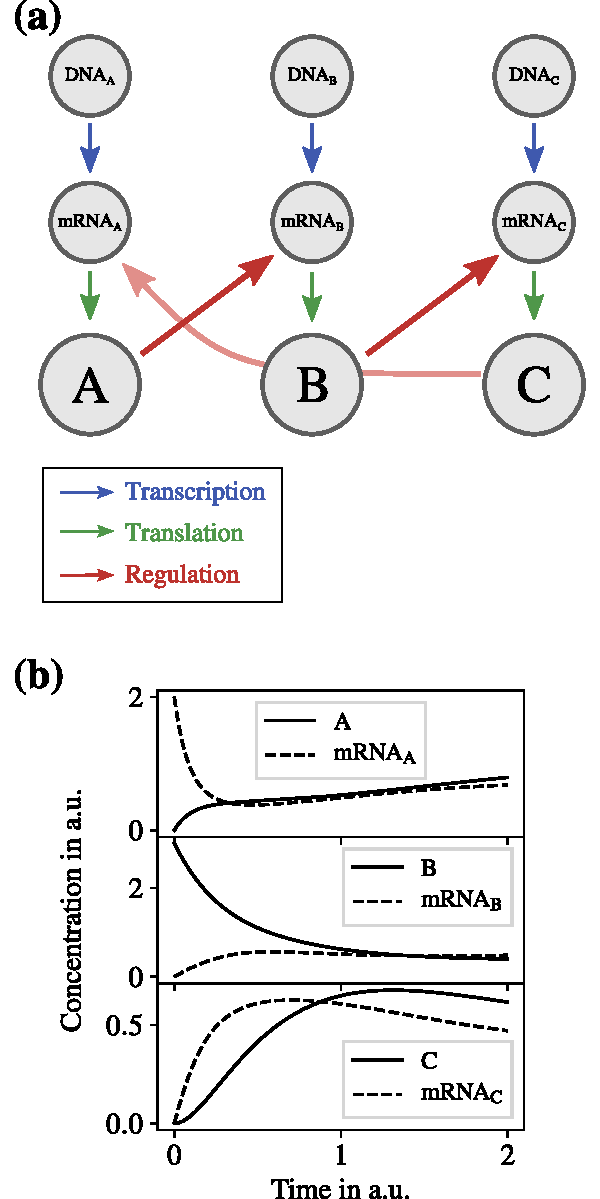
\includegraphics[width=.5\textwidth]{./figures_tex/scheme.pdf}
        \caption{The regulation network example described in Sec.~\ref{sec:generegulation}. \textbf{(a)}: Each circle depicts a species, each arrow corresponds to one reaction. Blue arrows denote transcription from DNA to $\mathrm{mRNA}$, green arrows denote translation from $\mathrm{mRNA}$ to protein, and red arrows denote the regulatory network. \textbf{(b)}: Concentration timeseries generated from the reaction network shown in~(a). The initial condition prescribes positive concentration values only for $\mathrm{B}$ protein and $\mathrm{mRNA}_\mathrm{A}$ species. This initial condition is used in the subsequent sections for further analysis.}
        \label{fig:network}
    \end{figure}

	\section{Results}\label{sec:results}
	
	The proposed estimation method is designed to find reaction networks and rates from experimental data. In the following the method is applied to data generated from the example described in Section \ref{sec:generegulation}.

	First it is assumed that the concentration data can be obtained without noise and it is shown that while the minimization problem (\ref{method:minimizationproblem}) without regularization, i.e., $\alpha=0$, yields rates that fit well to the input data, the original rates cannot be recovered while adding $L_1$ regularization and applying a cutoff recovers the underlying reaction network \textcolor{red}{(and rates?)}.
	
	In Section \ref{sec:case-2} the example data was generated using the Gillespie SSA \textbf{[cite]}. While the concentrations now contain stochastic noise, it is assumed that the initial state can be reproduced exactly and multiple measurements with that exact initial condition can be performed. It is shown that in the limit of many measurements a good fit can reliably be obtained.
	
	The last example is described in Section \ref{sec:case-3} and is an extension of the situation in Section \ref{sec:case-2} to multiple initial conditions. Due to more varied data and more statistics a good fit can be obtained with fewer measurements than in the case of just one initial condition.
	
	%measurement scenarios are considered that differ in how many time series are available and the level of noise that the data is subject to:
	%\begin{enumerate}
	%	\item The initial state of the measurement apparatus can be reproduced exactly. There is only one set of generating reaction rates. Each frame of a time series is subject to noise. The outcome of this scenario is one time series of concentrations with a certain noise-level.
	%	\item The process is observed multiple times. The initial state of the measurement apparatus differs in each observation. The outcome of this scenario is multiple time series each with a certain noise level and different initial states.
	%\item The process is observed multiple times. The initial state of the measurement apparatus differs in each observation. Additionally the generating reaction rates differ slightly in each observation. The outcome of this scenario is multiple time series each with a given noise level, different initial states and slightly perturbed underlying reaction rates.
	%\end{enumerate}

	\subsection{The noiseless case}\label{sec:case-1}
	
	In this section noiseless data generated from the law of mass action system described in Section \ref{sec:generegulation} is applied to the minimization problem (\ref{method:minimizationproblem}). When setting the hyperparameter $\alpha=0$ one obtains least squares regression with a constraint on the non-negativity of the estimated reaction rates.
	
	When applying no regularization, one can observe in Figure \ref{fig:case-1-sparsity-pattern} that the sparsity pattern does not match the generating reaction network and the reaction responsible for the decay of $\mathrm{A}$ particles is completely ignored. For a suitable choice of hyperparameters $\alpha \approx 1.91\cdot 10^{-7}$, $\lambda=1$, and a cutoff $\kappa = 0.22$ a sparser solution can be obtained and also the decay reaction as indicated by the red rings in the figure can be recovered. The cutoff $\kappa$ is applied so that for all reactions with an estimated rate $\hat{\xi} < \kappa$ a rate of $\hat{\xi} = 0$ is assigned. A bubble whose size corresponds to a rate of $\kappa$ is depicted in Fig.~\ref{fig:case-1-sparsity-pattern} in green.
	
	\begin{figure}
		\centering
		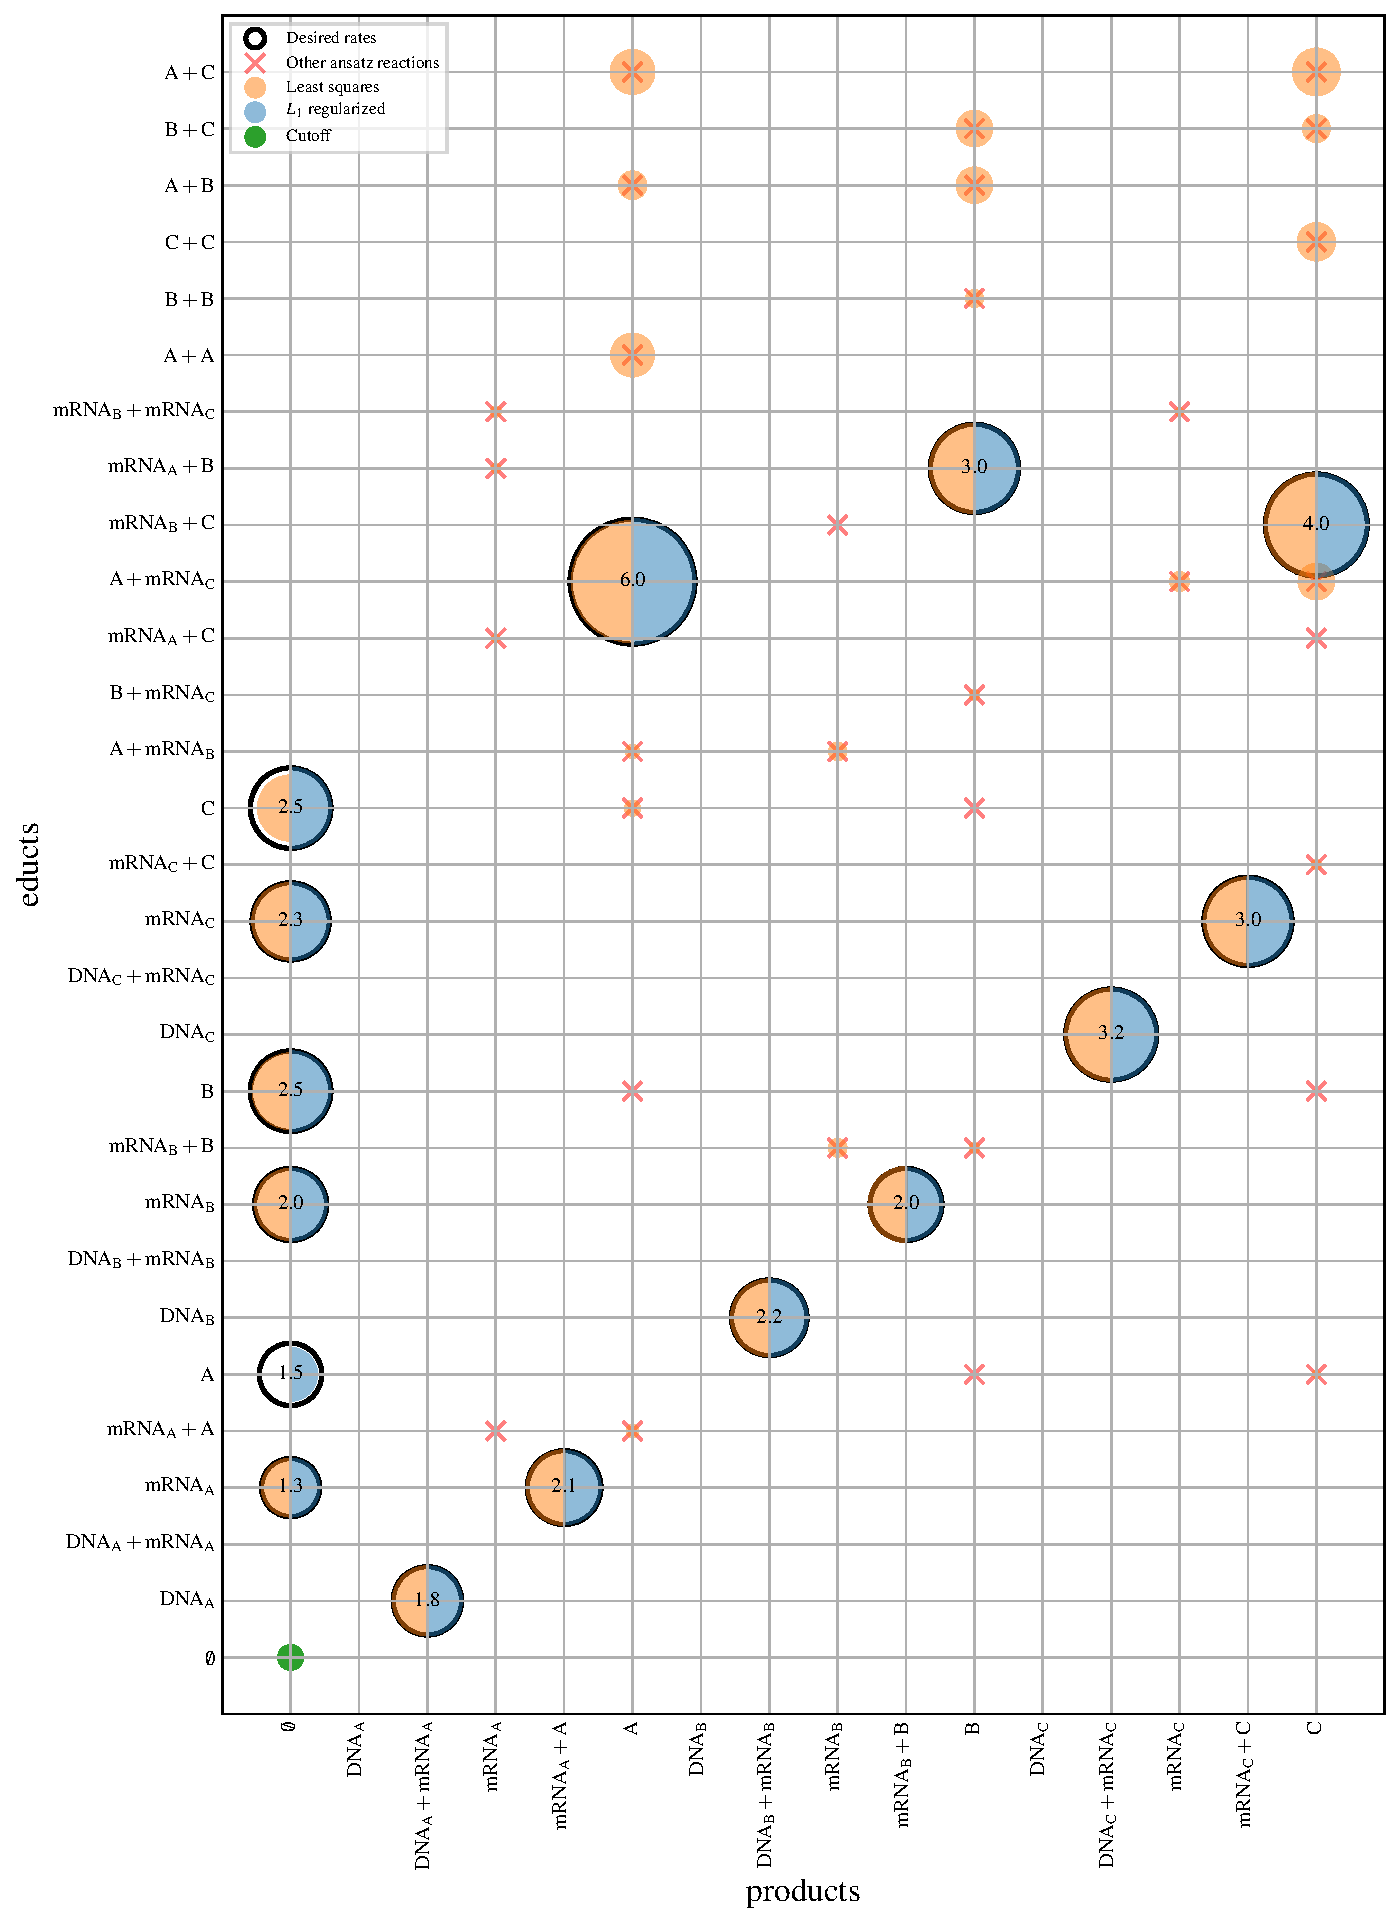
\includegraphics[width=.9\textwidth]{./figures_tex/sparsity_pattern}
		\caption{Estimated reaction rates in the system described in Sec.~\ref{sec:case-1}. The y and x axes contain reaction educts and products, respectively. A circle at position $(i,j)$ represents a reaction $i\rightharpoonup j$ whose rate has a linear relation with the area of the circle. The black outlines denote the reactions with which the system was generated and contain the respective rate value. Red crosses denote reactions that were used as additional ansatz reactions. Blue circles are estimated by linear least-squares and orange circles depict rates which were obtained by solving the minimization problem (\ref{method:minimizationproblem}). The latter rates are subject to a cutoff $\kappa=0.22$ corresponding to the green circle's area under which a sparse solution with the correct processes can be recovered. If a certain rate was estimated in both cases, two wedges instead of one circle are displayed.}
		\label{fig:case-1-sparsity-pattern}
	\end{figure}

	
	
	\subsection{Multiple measurements at the same noise level}\label{sec:case-2}
	
	\begin{itemize}
		\item Same setup as in Section \ref{sec:case-1}
		\item Cross validation with a shuffle split and 3 folds
		\item comparison to LSQ: LSQ unreliable
		\item in the limit of small noise one gets a good fit
		\item obtain cutoff in noise free case, compute failure rate (number of false positives and negatives)
	\end{itemize}

	\begin{figure}
		\centering
		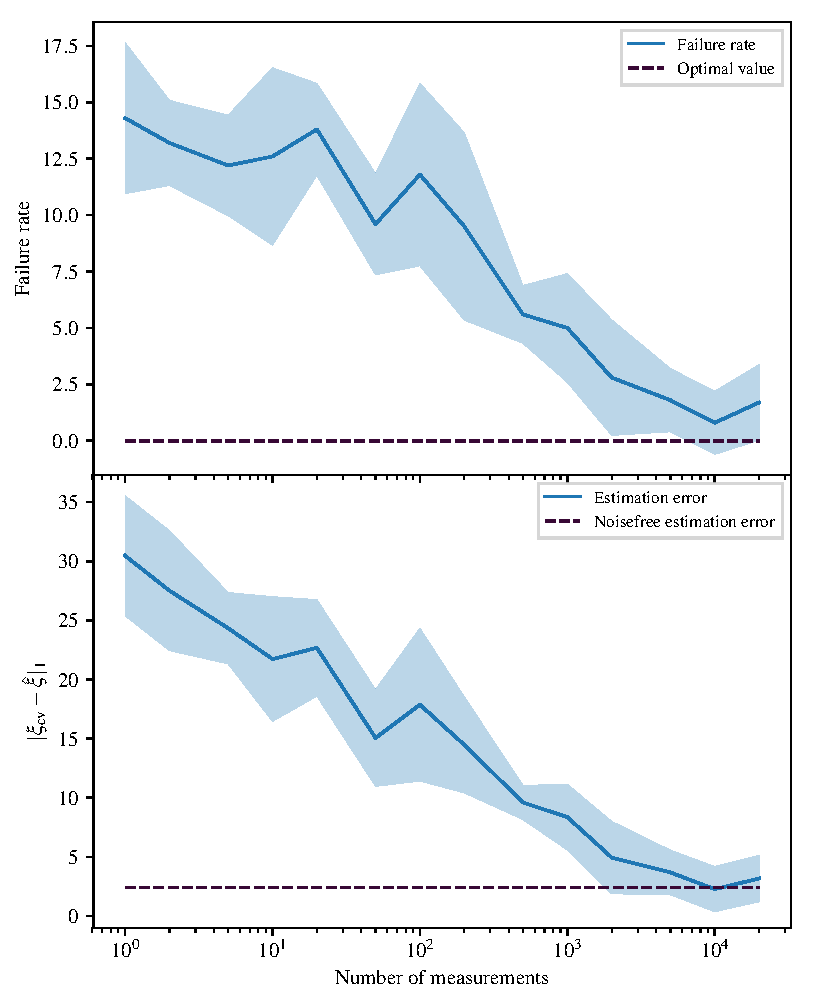
\includegraphics[width=.5\columnwidth]{./figures_tex/case2}
		\caption{Convergence of the estimation error when estimating the system described in Sec.~\ref{sec:case-1} with decreasing levels of noise by application of the minimization problem (\ref{method:minimizationproblem}). The level of noise is regulated by the number of measurements being averaged. The hyperparameters for each level of noise were estimated using 10-fold cross validation. This was repeated 10 times giving rise to the mean and standard deviation depicted by dark blue graph and shaded blue area, respectively. The failure rate is the number of incorrectly identified processes. The estimation error is given by the $L_1$ difference of the generating reaction rates $\hat{\xi}$ and the estimated reaction rates $\xi_\mathrm{CV}$.}
		\label{fig:case2-convergence}
	\end{figure}

	\subsection{Multiple initial conditions}\label{sec:case-3}
	
	\begin{itemize}
		\item extend situation of Section \ref{sec:case-3} to multiple initial conditions
		\item compute failure rate
	\end{itemize}

	\begin{figure}
		\centering
		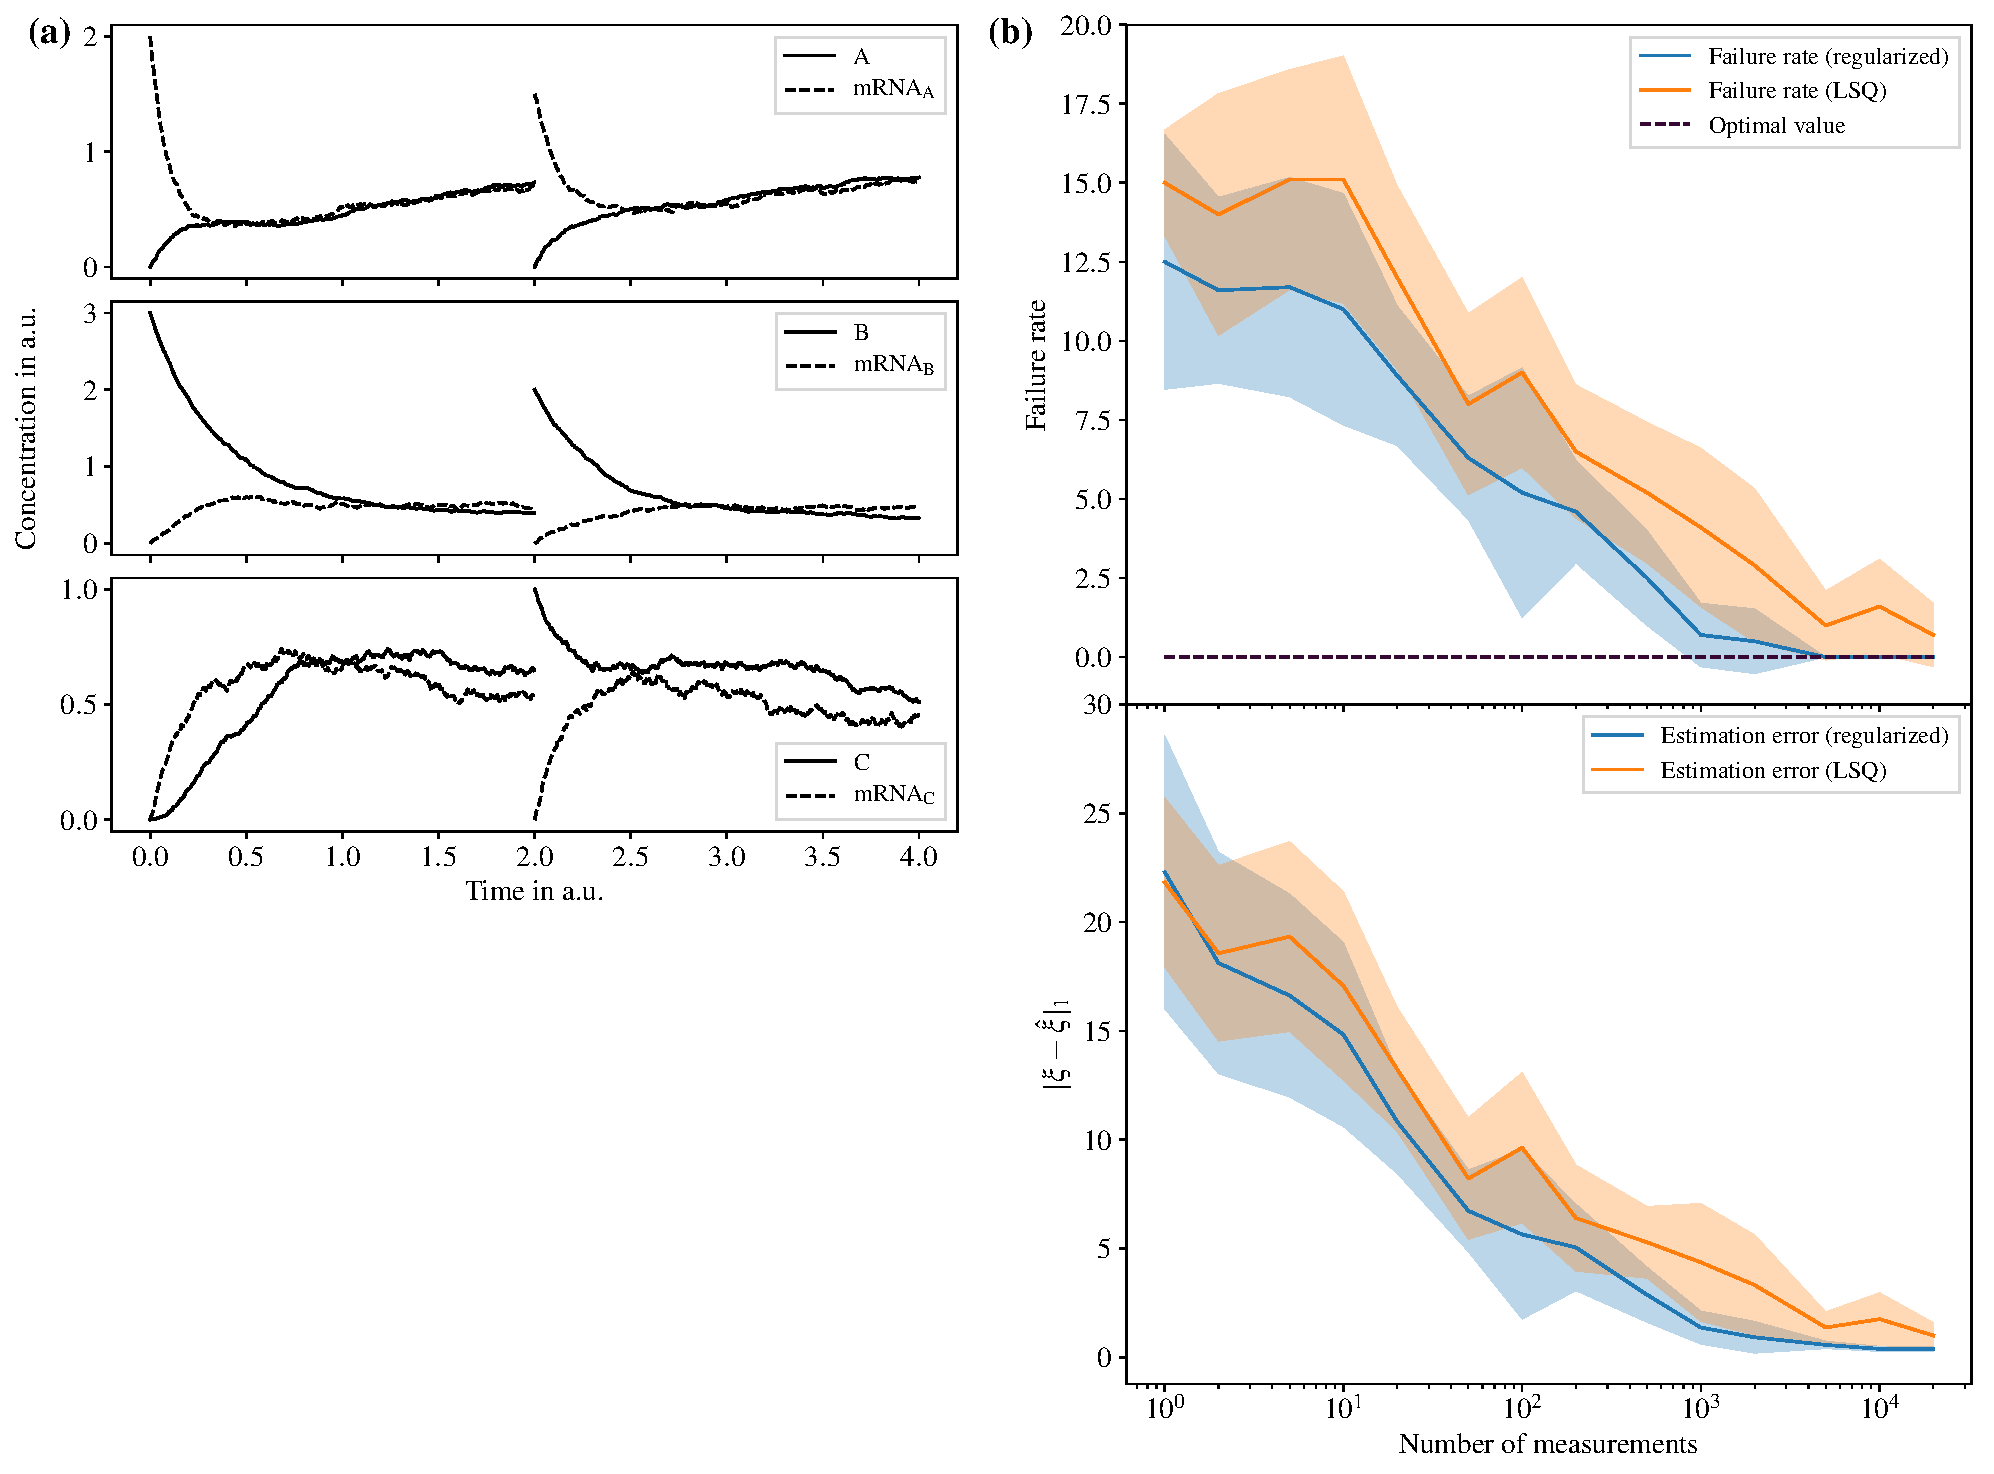
\includegraphics[width=\columnwidth]{./figures_tex/case3}
		\caption{Convergence of the estimation error when using two concatenated concentration timeseries with different initial conditions. \textbf{(a)}: A realization of one of the initial conditions that were used. It is identical to the initial conditions used in Sec.~\ref{sec:case-1} and Sec.~\ref{sec:case-2}. \textbf{(b)}: A realization of the other initial condition that was used. It prescribes positive initial concentrations for $\mathrm{mRNA}_\mathrm{A}$, $\mathrm{B}$, and $\mathrm{C}$ species. \textbf{(c)}: Analogously to Fig.~\ref{fig:case2-convergence} with the difference that 20-fold cross validation was used for hyperparameter estimation.}
	\end{figure}
    
	\section{Conclusion}
	\begin{colbox}{F8E0E0}
		todo
	\end{colbox}
	In this work we have successfully applied and extended the SINDy method to not only parsimoniously detect potentially nonlinear terms in a dynamical system from noisy data, but also yield, in this case, a sparse set of rates with respect to generating reactions (\ref{method:the-reactions}).

	In two examples it was demonstrated that despite noisy data and unavailable derivative measurements, a parsimonious generating reaction network that is qualitatively able to explain the observed data can be estimated.
	In particular it was shown in the first example that if there is no ambiguity in the underlying model and ansatz reaction library, the actual rates can be recovered with decreasing time step, i.e., increasing resolution of the jump process.
	In the second example we could obtain an even simpler model than what was used to generate data by making use of sparse regression and cross-validation.

	\newpage
% 	\bibliographystyle{alpha}
	\bibliographystyle{abbrv}
	\bibliography{bibliography.bib}
	\newpage	
	\section{Appendix}\label{sec:appendix}
	\begin{table}[h]
		\centering
		\scalebox{.75}{
			\begin{tabular}{rclcc}
				\multicolumn{3}{c}{Reaction} & rate & description \\ \hline\noalign{\vskip .1cm}
				$\mathrm{DNA}_\mathrm{A}$ &$\rightharpoonup$& $\mathrm{DNA}_\mathrm{A} + \mathrm{mRNA}_\mathrm{A}$ & $k_1 = 1.8$ & transcription of $\mathrm{mRNA}_\mathrm{A}$\\
				$\mathrm{mRNA}_\mathrm{A}$ &$\rightharpoonup$& $\mathrm{mRNA}_\mathrm{A} + \mathrm{A}$ & $k_2 = 2.1$ & translation of $\mathrm{A}$ proteins\\
				$\mathrm{mRNA}_\mathrm{A}$ &$\rightharpoonup$& $\emptyset$ & $k_3 = 1.3$ & $\mathrm{mRNA}_\mathrm{A}$ decay\\
				$\mathrm{A}$ &$\rightharpoonup$& $\emptyset$ & $k_4 = 1.5$ & decay of $\mathrm{A}$ proteins\\
				$\mathrm{DNA}_\mathrm{B}$ &$\rightharpoonup$& $\mathrm{DNA}_\mathrm{B} + \mathrm{mRNA}_\mathrm{B}$ & $k_5 = 2.2$ & transcription of $\mathrm{mRNA}_\mathrm{B}$\\
				$\mathrm{mRNA}_\mathrm{B}$ &$\rightharpoonup$& $\mathrm{mRNA}_\mathrm{B} + \mathrm{B}$ & $k_6 = 2.0$ & translation of $\mathrm{B}$ proteins\\
				$\mathrm{mRNA}_\mathrm{B}$ &$\rightharpoonup$& $\emptyset$ & $k_7 = 2.0$ & $\mathrm{mRNA}_\mathrm{B}$ decay\\
				$\mathrm{B}$ &$\rightharpoonup$& $\emptyset$ & $k_8 = 2.5$ & decay of $\mathrm{B}$ proteins\\
				$\mathrm{DNA}_\mathrm{C}$ &$\rightharpoonup$& $\mathrm{DNA}_\mathrm{C} + \mathrm{mRNA}_\mathrm{C}$ & $k_9 = 3.2$ & transcription of $\mathrm{mRNA}_\mathrm{C}$\\
				$\mathrm{mRNA}_\mathrm{C}$ &$\rightharpoonup$& $\mathrm{mRNA}_\mathrm{C} + \mathrm{C}$ & $k_{10} = 3.0$ & translation of $\mathrm{C}$ proteins\\
				$\mathrm{mRNA}_\mathrm{C}$ &$\rightharpoonup$& $\emptyset$ & $k_{11} = 2.3$ & $\mathrm{mRNA}_\mathrm{C}$ decay\\
				$\mathrm{C}$ &$\rightharpoonup$& $\emptyset$ & $k_{12} = 2.5$ & decay of $\mathrm{C}$ proteins\\
				$\mathrm{mRNA}_\mathrm{A} + \mathrm{A}$ &$\rightharpoonup$& $\mathrm{A}$ & $k_{13} = 0$ & self regulation of $\mathrm{A}$ proteins\\
				$\mathrm{mRNA}_\mathrm{B} + \mathrm{B}$ &$\rightharpoonup$& $\mathrm{B}$ & $k_{14} = 0$ & self regulation of $\mathrm{B}$ proteins\\
				$\mathrm{mRNA}_\mathrm{C} + \mathrm{C}$ &$\rightharpoonup$& $\mathrm{C}$ & $k_{15} = 0$ & self regulation of $\mathrm{C}$ proteins\\
				$\mathrm{mRNA}_\mathrm{B} + \mathrm{A}$ &$\rightharpoonup$& $\mathrm{A}$ & $k_{16} = 0$ & cyclic regulation of $\mathrm{A}$ proteins\\
				$\mathrm{mRNA}_\mathrm{C} + \mathrm{B}$ &$\rightharpoonup$& $\mathrm{B}$ & $k_{17} = 0$ & cyclic regulation of $\mathrm{B}$ proteins\\
				$\mathrm{mRNA}_\mathrm{A} + \mathrm{C}$ &$\rightharpoonup$& $\mathrm{C}$ & $k_{18} = 0$ & cyclic regulation of $\mathrm{C}$ proteins\\
				$\mathrm{mRNA}_\mathrm{C} + \mathrm{A}$ &$\rightharpoonup$& $\mathrm{A}$ & $k_{16} = 6.0$ & cyclic regulation of $\mathrm{A}$ proteins\\
				$\mathrm{mRNA}_\mathrm{B} + \mathrm{C}$ &$\rightharpoonup$& $\mathrm{C}$ & $k_{17} = 4.0$ & cyclic regulation of $\mathrm{C}$ proteins\\
				$\mathrm{mRNA}_\mathrm{A} + \mathrm{B}$ &$\rightharpoonup$& $\mathrm{B}$ & $k_{18} = 3.0$ & cyclic regulation of $\mathrm{B}$ proteins\\
				$\mathrm{mRNA}_\mathrm{A} + \mathrm{A}$ &$\rightharpoonup$& $\mathrm{mRNA}_\mathrm{A}$ & $k_{19} = 0$ & artificial fusion\\
				$\mathrm{mRNA}_\mathrm{B} + \mathrm{B}$ &$\rightharpoonup$& $\mathrm{mRNA}_\mathrm{B}$ & $k_{20} = 0$ & artificial fusion\\
				$\mathrm{mRNA}_\mathrm{A} + \mathrm{B}$ &$\rightharpoonup$& $\mathrm{mRNA}_\mathrm{A}$ & $k_{21} = 0$ & artificial fusion\\
				$\mathrm{mRNA}_\mathrm{B} + \mathrm{C}$ &$\rightharpoonup$& $\mathrm{mRNA}_\mathrm{B}$ & $k_{22} = 0$ & artificial fusion\\
				$\mathrm{mRNA}_\mathrm{C} + \mathrm{A}$ &$\rightharpoonup$& $\mathrm{mRNA}_\mathrm{C}$ & $k_{23} = 0$ & artificial fusion\\
				$\mathrm{mRNA}_\mathrm{A} + \mathrm{C}$ &$\rightharpoonup$& $\mathrm{mRNA}_\mathrm{A}$ & $k_{24} = 0$ & artificial fusion\\
				$\mathrm{mRNA}_\mathrm{B} + \mathrm{A}$ &$\rightharpoonup$& $\mathrm{mRNA}_\mathrm{B}$ & $k_{25} = 0$ & artificial fusion\\
				$\mathrm{A} + \mathrm{A}$ &$\rightharpoonup$& $\mathrm{A}$ & $k_{26} = 0$ & $\mathrm{A}$ regulates $\mathrm{A}$\\
				$\mathrm{B} + \mathrm{B}$ &$\rightharpoonup$& $\mathrm{B}$ & $k_{27} = 0$ & $\mathrm{B}$ regulates $\mathrm{B}$\\
				$\mathrm{C} + \mathrm{C}$ &$\rightharpoonup$& $\mathrm{C}$ & $k_{28} = 0$ & $\mathrm{C}$ regulates $\mathrm{C}$\\
				$\mathrm{B} + \mathrm{A}$ &$\rightharpoonup$& $\mathrm{A}$ & $k_{29} = 0$ & artificial fusion between proteins\\
				$\mathrm{C} + \mathrm{B}$ &$\rightharpoonup$& $\mathrm{B}$ & $k_{30} = 0$ & artificial fusion between proteins\\
				$\mathrm{A} + \mathrm{C}$ &$\rightharpoonup$& $\mathrm{C}$ & $k_{31} = 0$ & artificial fusion between proteins\\
				$\mathrm{C} + \mathrm{A}$ &$\rightharpoonup$& $\mathrm{A}$ & $k_{32} = 0$ & artificial fusion between proteins\\
				$\mathrm{B} + \mathrm{C}$ &$\rightharpoonup$& $\mathrm{C}$ & $k_{33} = 0$ & artificial fusion between proteins\\
				$\mathrm{A} + \mathrm{B}$ &$\rightharpoonup$& $\mathrm{B}$ & $k_{34} = 0$ & artificial fusion between proteins\\
				$\mathrm{A}$ &$\rightharpoonup$& $\mathrm{B}$ & $k_{35} = 0$ & artificial conversion between proteins\\
				$\mathrm{B}$ &$\rightharpoonup$& $\mathrm{C}$ & $k_{36} = 0$ & artificial conversion between proteins\\
				$\mathrm{C}$ &$\rightharpoonup$& $\mathrm{A}$ & $k_{37} = 0$ & artificial conversion between proteins\\
				$\mathrm{A}$ &$\rightharpoonup$& $\mathrm{C}$ & $k_{38} = 0$ & artificial conversion between proteins\\
				$\mathrm{C}$ &$\rightharpoonup$& $\mathrm{B}$ & $k_{39} = 0$ & artificial conversion between proteins\\
				$\mathrm{B}$ &$\rightharpoonup$& $\mathrm{A}$ & $k_{40} = 0$ & artificial conversion between proteins\\
				$\mathrm{mRNA}_\mathrm{B} + \mathrm{mRNA}_\mathrm{C}$ &$\rightharpoonup$& $\mathrm{mRNA}_\mathrm{A}$ & $k_{41} = 0$ & artificial fusion\\
				$\mathrm{mRNA}_\mathrm{C} + \mathrm{mRNA}_\mathrm{B}$ &$\rightharpoonup$& $\mathrm{mRNA}_\mathrm{C}$ & $k_{42} = 0$ & artificial fusion\\
				$\mathrm{mRNA}_\mathrm{C} + \mathrm{A}$ &$\rightharpoonup$& $\mathrm{C}$ & $k_{43} = 0$ & artificial fusion\\
				$\mathrm{mRNA}_\mathrm{C} + \mathrm{C}$ &$\rightharpoonup$& $\mathrm{C}$ & $k_{43} = 0$ & artificial fusion
			\end{tabular}
		}
		\caption{Full set of ansatz reactions $\Theta$ used in Sec.~\ref{sec:results}.}
		\label{tab:reaction-library}
	\end{table}
\end{document}
